\documentclass{article}
\usepackage{amsmath,tkz-tab}
\begin{document}
 \begin{center}
 \LARGE\color{blue}\fcolorbox{red}{yellow!10}{$f(x)=\sin (x)$}
 \end{center}
 %%%%%%%%%%%%%%%%%%%%% tv %%%%%%%%%%%%%%%%%%%%%%
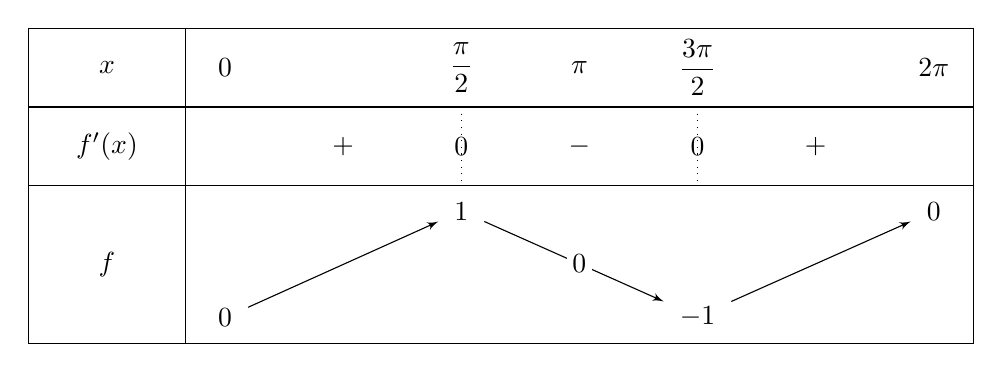
\begin{tikzpicture}
 \tkzTabInit{$x$/1,$f'(x)$/1,$f$/2}{$0$,$\dfrac{\pi}{2}$,$\dfrac{3\pi}{2}$,$2\pi$}
 \tkzTabLine{,+,z,-,z,+,}
 \tkzTabVar{-/$0$,+/$1$,-/$-1$,+/$0$}
 \tkzTabVal{2}{3}{0.5}{$\pi$}{0}
\end{tikzpicture}
\end{document}